% Original book diagram: fig:dbn-filtering
% Book source: sections/Part_III/prob_robotics_foundations.tex
% Original diagram authorship retained. Visual design: Ziad Mosalam.
\documentclass[11pt,border=8pt]{standalone}
\usepackage{amsmath,amssymb,graphicx,tikz}
\usetikzlibrary{arrows.meta,automata,positioning,calc,shapes.geometric,fit,backgrounds,patterns}
\newcommand{\vect}[1]{\mathbf{#1}}
\newcommand{\mat}[1]{\mathbf{#1}}
\newcommand{\Normal}{\mathcal{N}}
\newcommand{\prob}{p}
\newcommand{\E}{\mathbb{E}}
\newcommand{\Var}{\mathrm{Var}}
\newcommand{\Cov}{\mathrm{Cov}}
\newcommand{\CovP}{\mathbf{P}}
\newcommand{\Prob}{\mathbb{P}}
\setlength{\textwidth}{6.5in}
% Shared visual vocabulary for the book's original diagrams.
% Figures opt in explicitly, so unrelated text and existing additions are unchanged.
\definecolor{BookBlue}{HTML}{003262}
\definecolor{BookGold}{HTML}{B17A00}
\definecolor{BookTeal}{HTML}{247C86}
\definecolor{BookInk}{HTML}{30363B}
\definecolor{BookLight}{HTML}{E9EFF5}
\tikzset{
  book figure/.style={font=\small\rmfamily, color=BookBlue, text=BookInk,
    line width=0.8pt, >=Latex},
  book axis/.style={->, draw=BookInk, line width=0.6pt},
  book link/.style={->, draw=BookBlue, line width=0.8pt},
  book observation/.style={draw=BookGold, fill=BookGold!8},
  book state/.style={draw=BookBlue, fill=BookLight},
  book note/.style={font=\footnotesize\rmfamily, text=BookInk}
}

\begin{document}
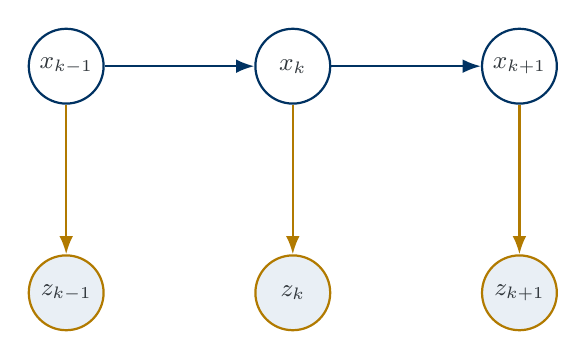
\begin{tikzpicture}[font=\small, text=BookInk, draw=BookBlue, line width=0.8pt, >=Latex,
    >=Latex,
    node distance=2.8cm and 1.9cm,
    every node/.style={font=\small},
    state/.style={
        circle,
        draw=BookBlue, fill=white,
        minimum size=9.5mm,
        inner sep=1pt,
        line width=0.8pt
    },
    meas/.style={
        circle,
        draw=BookBlue, fill=white,
        fill=BookLight, draw=BookGold,
        minimum size=9.5mm,
        inner sep=1pt,
        line width=0.8pt
    },
    arrow/.style={->, line width=0.8pt}
]

\node[state] (x1) {$x_{k-1}$};
\node[state, right=of x1] (x2) {$x_k$};
\node[state, right=of x2] (x3) {$x_{k+1}$};

\node[meas, below=1.9cm of x1] (y1) {$z_{k-1}$};
\node[meas, below=1.9cm of x2] (y2) {$z_k$};
\node[meas, below=1.9cm of x3] (y3) {$z_{k+1}$};

\draw[arrow] (x1) -- (x2);
\draw[arrow] (x2) -- (x3);

\draw[arrow,draw=BookGold] (x1) -- (y1);
\draw[arrow,draw=BookGold] (x2) -- (y2);
\draw[arrow,draw=BookGold] (x3) -- (y3);

\end{tikzpicture}
\end{document}
